\documentclass[12pt]{article}
\usepackage[utf8]{inputenc}
\usepackage[left=2.5cm, top=1.5cm, right=2.5cm, bottom=2cm, a4paper]{geometry}
\usepackage{polski}
\usepackage{fancyhdr}
\usepackage{lastpage}
\usepackage{amsmath}
\usepackage{amssymb}
\usepackage{bbm}
\usepackage{amsthm}
\usepackage{wrapfig}
\usepackage{indentfirst}
\usepackage[absolute,overlay]{textpos}
\usepackage{centernot}
\usepackage{tikz}
\usetikzlibrary{calc}
\usepackage{hyperref}
\hypersetup{
    colorlinks,
    citecolor=black,
    filecolor=black,
    linkcolor=black,
    urlcolor=black
}
\usepackage{array}                          % for \newcolumntype macro
\newcolumntype{L}{>{$\displaystyle}l<{$}}   % math-mode version of "l" column type

\newcommand{\zset}{\mathbb{Z}}
\newcommand{\zplus}{\mathbb{Z}_+}
\newcommand{\nat}{\mathbb{N}}
\newcommand{\real}{\mathbb{R}}
\newcommand{\rplus}{\mathbb{R}_+}
\renewcommand{\tan}{\operatorname{tg}}
\renewcommand{\arctan}{\operatorname{arctg}}

\newcommand{\eqline}{\noalign{\smallskip} \hline \noalign{\smallskip}}

\newtheorem*{theorem*}{Twierdzenie}
\newtheorem*{lemma*}{Lemat}
\newtheorem{theorem}{Twierdzenie}
\newtheorem{lemma}{Lemat}
% Set title:
% \begin{lemma*}[Title]

\setlength{\parindent}{1.25cm}
\AddToHook{cmd/section/before}{\clearpage}
\graphicspath{{images/}}

% Pagination
\pagestyle{fancy}
\fancyhf{}
\renewcommand{\headrulewidth}{0pt}
\cfoot{
Strona $\thepage$ z $\pageref{LastPage}$
}
% Text in a specified place:
% {block width} (coords) 
% \begin{textblock*}{5cm}(10cm,6cm)
%    Your text here
% \end{textblock*}

\title{Egzamin z Analizy Matematycznej}
\author{2023/2024}
\date{29 stycznia 2024}
\setcounter{section}{-1}

\begin{document}
\maketitle 
\tableofcontents

\section{Wstęp} \label{wstep}
\subsection{Od autora rozwiązań} 
Dokument zawiera rozwiązania do wszystkich zadań z egzaminu podstawowego z Analizy Matematycznej z 2024 roku na kierunku Informatyka. Każda sekcja dotycząca konkretnego zadania składa się z 3 podsekcji -- treści zadania, rozwiązania i potwierdzenia rozwiązania (w formie rozwiązania przez jakiś program, np. Wolfram Alpha, lub fragmentu prezentacji wykładowej). Po dokumencie można poruszać się klikając odpowiednią nazwę sekcji bądź podsekcji w spisie treści.

Jeśli masz jakieś uwagi lub znajdziesz błędy w którymś z rozwiązań, zgłoś je w sekcji Issues wraz z wyjaśnieniem. Możesz również samemu poprawić rozwiązanie zgłaszając Pull request -- także z wyjaśnieniem (proszę edytować jedynie plik .tex).
\subsection{Skan egzaminu}
\includegraphics{am24.png}

\section{Zadanie 1}
\subsection{Treść zadania}
(a)$(1p)$ Podaj warunek konieczny istnienia pochodnej właściwiej funkcji $f(x)$ w $x=x_0$.

(b)$(2p)$ Korzystając z definicji, oblicz pochodną funkcji $f(x) = \sqrt{x-2}$.

(c)$(5p)$ Znajdź punkty przegięcia i zbadaj wklęsłość/wypukłość wykresu funkcji 
\[f(x) = (2 - \ln x) \cdot x^2\]

\subsection{Rozwiązanie}
(a) Jeżeli istnieje pochodna właściwa funkcji $f(x)$ w punkcie $x=x_0$, to funkcja $f(x)$ jest ciągła w punkcie $x=x_0$.

(b)
\begin{align*}
    f'(x) &= \lim_{h\to0} \frac{f(x+h) - f(x)}{h} \\
    f'(x) &= \lim_{h\to0} \frac{\sqrt{x+h-2} - \sqrt{x-2}}{h}, \quad D_{f} = [2,\infty) \\
    f'(x) &= \lim_{h\to0} \frac{\sqrt{x+h-2} - \sqrt{x-2}}{h} \cdot \frac{\sqrt{x+h-2} + \sqrt{x-2}}{\sqrt{x+h-2} + \sqrt{x-2}} \\
    f'(x) &= \lim_{h\to0} \frac{x+\centernot{h}-2-x+2}{\centernot{h}(\sqrt{x+h-2} + \sqrt{x-2})} \\
    f'(x) &= \lim_{h\to0} \frac{1}{\sqrt{x+h-2} + \sqrt{x-2})} \\   
    f'(x) &= \frac{1}{\sqrt{x+0-2} + \sqrt{x-2})} \\    
    f'(x) &= \frac{1}{2\sqrt{x-2}}, \quad D_{f'} = (2,\infty)
\end{align*}

(c)
\begin{align*}
    f(x) &= (2-\ln x)x^2 = 2x^2 - x^2\ln x, \quad D_{f} = (0,\infty) \\
    f'(x) &= 4x - 2x\ln x - \frac{x^2}{x} = 3x - 2x \ln x, \quad D_{f'} = (0,\infty) \\
    f''(x) &= 3 - 2 \ln x - \frac{2x}{x} = 1 - 2 \ln x, \quad D_{f''} = (0,\infty) \\
\end{align*}
\begin{align*}
\begin{aligned}[c]
    f \text{  wypukła} \iff& f''(x) > 0 \\
    1-2\ln x &> 0 \\ 
    \frac{1}{2} &> \ln x \\
    \sqrt{e} &> x
\end{aligned}
\quad\quad\quad
\begin{aligned}[c]
    f \text{  wklęsła} \iff& f''(x) < 0 \\
    1-2\ln x &< 0 \\ 
    \frac{1}{2} &< \ln x \\
    \sqrt{e} &< x
\end{aligned} \\
\end{align*}

Punkt przegięcia w $x_0$ występuje, kiedy $f''(x_0) = 0$ i $f''$ zmienia znak w otoczeniu $x_0$. $f''(x_0) = 0 \iff x_0 = \sqrt{e}$, a wiemy, na podstawie wcześniej wyliczonych nierówności, że druga pochodna zmienia znak w otoczeniu tego punktu.

Podsumowując:
Punkt przegięcia: $x_0 = \sqrt{e}$.
Funkcja jest wypukła w przedziale $(0,\sqrt{e})$.
Funkcja jest wklęsła w przedziale $(\sqrt{e}, \infty)$.

\subsection{Potwierdzenie rozwiązania}
(a)

\includegraphics[scale=0.5]{am_1_a.png}

(b)

\includegraphics[scale=0.35]{am_1_b.png}

(c)

\includegraphics[scale=0.35]{am_1_c.png}

\section{Zadanie 2}
\subsection{Treść zadania}
Oblicz całki

(a)$(3p)$ $\displaystyle \int \frac{1}{3+\sin x+3\cos x} dx$

(b)$(3p)$ $\displaystyle \int \arccot \sqrt{x} \; dx$

\subsection{Rozwiązanie}
(a)

\begin{equation*}
    \begin{aligned}[c]
        &\int \frac{1}{3+\sin x+3\cos x} dx = \\
        &\int \frac{1}{3+\frac{2u}{1+u^2}+3\frac{1-u^2}{1+u^2}} \cdot \frac{2}{1+u^2}du = \\
        &\int \frac{2}{3(1+u^2)+2u+3(1-u^2)} du = \\
        &\int \frac{\centernot{2}}{3(\centernot{2})+\centernot{2}u} du = \\
        &\int \frac{1}{3 + u} du = \\
        &\ln |u+3| + C = \\
        &\ln \left|\tan\frac{x}{2} + 3\right| + C \\
        \text{\phantom{-}} \\ \text{\phantom{-}} \\ \text{\phantom{-}} \\ \text{\phantom{-}} \\
    \end{aligned} \quad\quad\quad
    \begin{aligned}[c]
        &u = \tan \frac{x}{2} \\
        &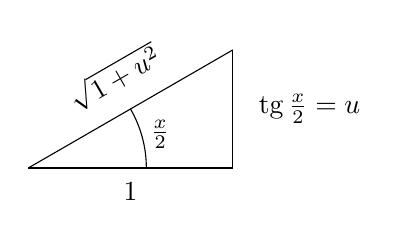
\begin{tikzpicture}[baseline=-0.65ex,scale=0.5]
            \draw (5.1962, 0) -- (5.1962, 3);
            \draw (0, 0) -- (5.1962, 0);
            \draw (0, 0) -- (5.1962, 3);
            \draw (3,0) arc (0:30:3);
            \node at (3.35, 0.85) {$\frac{x}{2}$};
            \node[rotate=30] at (2.5981 - 0.4, 1.5 + 0.8) {$\sqrt{1 + u^2}$};
            \node at (5.1962 + 1.95, 1.5) {$\tan\frac{x}{2} = u$};
            \node at (2.5981, -0.6) {$1$};
        \end{tikzpicture} \\
        &du = \frac{1}{\cos^2x} \cdot \frac{1}{2} dx\\
        &\frac{2}{1+u^2}du = dx\\
        &\sin x = 2\sin\frac{x}{2}\cos\frac{x}{2} \\
        &\sin x = \frac{2u}{1+u^2} \\
        &\cos x = \cos^2\frac{x}{2} - \sin^2\frac{x}{2} \\
        &\cos x = \frac{1-u^2}{1+u^2}\\        
    \end{aligned}
\end{equation*}

(b) (Uwaga: $\arccot x = \pi/2 - \arctan x$, co wynika bezpośrednio z własności f. tryg.)

\begin{equation*}
    \begin{aligned}[c]
        &\int \arccot \sqrt{x} \; dx = \\
        &\int \left( \frac{\pi}{2} - \arctan \sqrt{x} \right) dx = \\
        & \frac{\pi}{2} x - \int 2t \arctan t \; dt = \\
        & \frac{\pi}{2} x - \left( t^2 \arctan t - \int \frac{t^2}{1+t^2} dt \right) = \\
        & \frac{\pi}{2} x - x \arctan \sqrt{x} + \int \frac{1+t^2-1}{1+t^2} dt = \\
        & \frac{\pi}{2} x - x \arctan \sqrt{x} + \int dt - \int\frac{1}{1+t^2} dt = \\
        & \frac{\pi}{2} x - x \arctan \sqrt{x} + t - \arctan t + C = \\
        & \frac{\pi}{2} x - x \arctan \sqrt{x} + \sqrt{x} - \arctan \sqrt{x} + C \\
    \end{aligned} \quad\quad\quad
    \begin{aligned}
        &t = \sqrt{x} \\    
        &t^2 = x \\    
        &2tdt = dx \\    
        &\text{\phantom{-}} \\
        &\begin{aligned}[c]
            u &= \arctan t \\
            du &= \frac{dt}{1+t^2} \\    
        \end{aligned} \quad
        \begin{aligned}[c]
            dv &= 2tdt\\
            v &= t^2 \\    
        \end{aligned} \\
        &\text{\phantom{-}} \\ &\text{\phantom{-}} \\ &\text{\phantom{-}} \\ &\text{\phantom{-}} \\ &\text{\phantom{-}} \\
    \end{aligned}
\end{equation*}

\subsection{Potwierdzenie rozwiązania}
(a)

\includegraphics[scale=0.4]{am_2_a.png}

Przy czym
\[ \ln \left|\sin \frac{x}{2} + 3 \cos \frac{x}{2}\right| - \ln \left|\cos \frac{x}{2}\right| = \ln\left|\frac{\sin \frac{x}{2} + 3 \cos \frac{x}{2}}{\cos \frac{x}{2}}\right| = \ln\left|\tan \frac{x}{2} + 3 \right|\]

(b) (Uwaga: w Wolframie jest zaimplementowana zła wersja (a mianowicie wersja nieciągła) funkcji $\arccot \alpha$, stąd do poprawnego obliczenia wyniku wymagane jest podstawienie na $\pi/2 - \arctan \alpha$)

\includegraphics[scale=0.4]{am_2_b.png}

\section{Zadanie 3}
\subsection{Treść zadania}
$(5p)$ Oblicz objętość bryły powstałej z obrotu wokół osi $OX$ obszaru ograniczonego przez $y=0$ i $\displaystyle y=\sqrt{\frac{x}{e^x}}$ dla $x \geq 0$.

\subsection{Rozwiązanie}
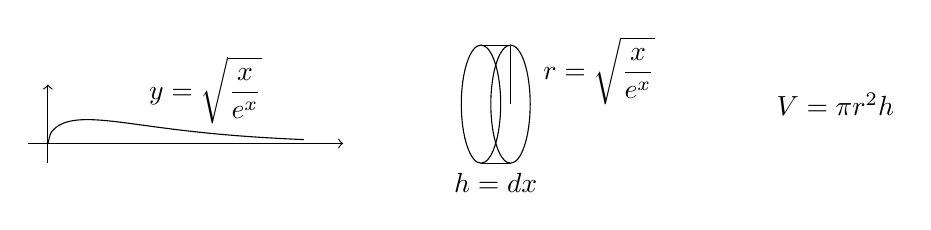
\begin{tikzpicture}[baseline=-0.65ex,scale=0.5]
    \node at (4, 1.35) {$\displaystyle y=\sqrt{\frac{x}{e^x}}$};
    \draw [smooth,samples=100,domain=0:6.5] plot(\x,{sqrt(\x/exp(\x))});
    \draw [->](0, -0.5) -- (0, 1.5);
    \draw [->](-0.5, 0) -- (7.5, 0);
    \draw (11, 1) ellipse (0.5 and 1.5);
    \draw (11.75, 1) ellipse (0.5 and 1.5);
    \draw (11.75, 1) -- (11.75, 2.5);
    \draw (11, 2.5) -- (11.75, 2.5);
    \draw (11, -0.5) -- (11.75, -0.5);
    \node at (11.375, -1) {$h=dx$};
    \node at (14, 1.85) {$r = \displaystyle \sqrt{\frac{x}{e^x}}$};
    \node at (20, 1) {$V = \pi r^2 h$};
\end{tikzpicture}

$\displaystyle y(0) = 0,\quad \lim_{x\to\infty}y=0\quad$

Poszukiwana objętość $\displaystyle = \pi\int_0^\infty \frac{x}{e^x} dx= (*)$

\begin{equation*}
    \begin{aligned}[c]
        &\int \frac{x}{e^x} dx = \int xe^{-x} dx = \\
        &-\frac{x}{e^x} - \int \left( -e^{-x} \right) dx = \\
        &-\frac{x}{e^x} - \frac{1}{e^x} + C = \\
        &\frac{-x-1}{e^x} + C
    \end{aligned} \quad\quad\quad
    \begin{aligned} 
        &\begin{aligned}[c]
            u &= x \\
            du &= 1 \\    
        \end{aligned} \quad
        \begin{aligned}[c]
            dv &= e^{-x}\\
            v &= -e^{-x} \\    
        \end{aligned} \\
        &\text{\phantom{-}} \\ &\text{\phantom{-}} \\ &\text{\phantom{-}} \\
    \end{aligned}
\end{equation*}

\[(*) = \pi\left(\lim_{x\to\infty}\stackrel{\text{L'Hôpital}}{\left(\frac{-x-1}{e^x}\right)} - \left(\frac{-0-1}{e^0}\right) \right) = \pi \left(\lim_{x\to\infty}\left(\frac{-1}{e^x}\right) -(-1)\right) = \pi (0 + 1) = \pi \]

\subsection{Potwierdzenie rozwiązania}
\includegraphics[scale=0.425]{am_3.png}

\section{Zadanie 4}
\subsection{Treść zadania}
(a)$(1p)$ Podaj warunek konieczny zbieżności nieskończonego szeregu liczbowego.

(b)$(4p)$ Znajdź przedział zbieżności szeregu
\[\sum_{n=4}^\infty (-1)^n\frac{(x-2)^n}{3^n\sqrt{n}}\]

\subsection{Rozwiązanie}
(a) Jeżeli nieskończony szereg liczbowy $\displaystyle \sum a_n$ jest zbieżny, to $\displaystyle \lim_{n\to\infty} a_n = 0$.

(b) Skorzystamy z kryterium Cauchy'ego zbieżności szeregów. Jeżeli granica odpowiadająca temu kryterium jest mniejsza niż jeden, to szereg jest zbieżny. Jeżeli jest równa jeden, to należy ten przypadek rozważyć oddzielnie. W pozostałych przypadkach szereg jest rozbieżny.

Niech $\displaystyle (-1)^n \frac{(x-2)^n}{3^n\sqrt{n}} = a_n$, wówczas
\begin{align*}
    \lim_{n\to\infty} \sqrt[n]{|a_n|} < 1 \\
    \lim_{n\to\infty} \sqrt[n]{|(-1)^n \frac{(x-2)^n}{3^n\sqrt{n}}|} < 1 \\
    \lim_{n\to\infty} \sqrt[n]{|(-1)|^n} \; \frac{\sqrt[n]{|x-2|^n}}{\sqrt[n]{3^n}\sqrt[n]{\sqrt{n}}} < 1 \\
    1 \; \frac{|x-2|}{3 \cdot 1} < 1 \\
    |x-2| < 3 \\
    -1 < x < 5 \\
\end{align*}
\begin{align*}
\begin{aligned}[c]
    x &= -1: \\
    a_n &= (-1)^n \frac{(-1-2)^n}{3^n\sqrt{n}} \\
    a_n &= \frac{(3)^n}{3^n\sqrt{n}} \\
    a_n &= \frac{1}{n^{\frac{1}{2}}} \\
    \text{Szereg} &\text{ Dirichleta o potędze} < 1\\
    &\implies \text{rozbieżny} \\
\end{aligned}
\quad\quad\quad
\begin{aligned}[c]
    x &= 5: \\
    a_n &= (-1)^n \frac{(5-2)^n}{3^n\sqrt{n}} \\
    a_n &= \frac{(-3)^n}{3^n\sqrt{n}} \\
    a_n &= (-1)^n\frac{1}{n^{\frac{1}{2}}} \\
    \text{Z kryt.} &\text{ Leibniza} \lim_{n\to\infty}a_n = 0 \land |a_{n+1}| < |a_{n}| \\
    &\implies \text{zbieżny} \\
\end{aligned} \\
\end{align*}

Przedział zbieżności szeregu wynosi $(-1, 5]$.
\pagebreak

\subsection{Potwierdzenie rozwiązania}
(a)

\includegraphics[scale=0.695]{am_4_a.png}

(b)

\includegraphics[scale=0.425]{am_4_b.png}

\section{Zadanie 5}
\subsection{Treść zadania}
Rozwiąż równania różniczkowe

(a)$(4p)$ $y''+2y' = 8xe^{-2x}$

(b)$(3p)$ $y' \sin x - y \cos x = (x \sin x)^2$

(c)$(2p)$ Naszkicuj obszar istnienia i jednoznaczności rozwiązań równania z punktu (b). Następnie określ na jakim maksymalnie przedziale może istnieć rozwiązanie tego równania z warunkiem początkowym $y(1) = 1$.

\subsection{Rozwiązanie}
(a) $y''+2y' = 8xe^{-2x}$

$CORN = CORJ + CSRN$

$CORJ:$
\begin{align*}
    r^2 + 2r &= 0 \\
    r = -2 &\lor r = 0 \\
    y_{CORJ} &= C_1 e^{-2x} + C_2 e^{0x} \\
    y_{CORJ} &= C_1 e^{-2x} + C_2 \\
\end{align*}

$CSRN \text{ (metodą przewidywań)}:$
\begin{align*}
    &y = (Ax + B)xe^{-2x}, \quad \text{(mnożymy przez dodatkowy $x$, ponieważ $-2$ jest jednym z $r$)} \\
    &y' = -2(Ax^2+Bx)e^{-2x} + (2Ax+B)e^{-2x} = (-2Ax^2-2Bx+2Ax+B)e^{-2x} \\
    &y'' = -2(-2Ax^2-2Bx+2Ax+B)e^{-2x} + (-4Ax-2B+2A)e^{-2x} \\
    &y'' = (4Ax^2+4Bx-8Ax-4B+2A)e^{-2x} \\
\end{align*}
\begin{align*}
    y''+2y' &= (4Ax^2+4Bx-8Ax-4B+2A)e^{-2x} + 2(-2Ax^2-2Bx+2Ax+B)e^{-2x} \\
    y''+2y' &= ((4A-4A)x^2+(4B-8A-4B+4A)x-4B+2A+2B)e^{-2x} \\
    y''+2y' &= (-4Ax-2B+2A)e^{-2x} \\
    &-4A = 8 \implies A=-2 \\
    &-2B+2A=0 \implies B=-2 \\
    &y_{CSRN} = (-2x^2-2x)e^{-2x}
\end{align*}

\[y_{CORN} = C_1 e^{-2x} + C_2 -2x^2e^{-2x} -2xe^{-2x} \]

(b) 
\begin{align*}
    y' \sin x - y \cos x &= (x \sin x)^2 \;\; | \div \sin x, \; \sin x \neq 0\\
    y'  - y \cot x &= x^2 \sin x \\
    \text{Czynnik całkujący: } \mu &= e^{\int (-\cot x) dx} = C_1 e^{-log|sinx|} = \frac{C_2}{sinx} \\
    \frac{C_2y'}{\sin x} + \frac{- C_2 y \cot x }{\sin x} &= C_2 x^2 \;\; | \div C_2 \\
    \frac{d}{dx} \left( \frac{y}{\sin x} \right) &= x^2 \\
    \int d \left( \frac{y}{\sin x} \right) &= \int x^2 dx \\
    \frac{y}{\sin x} &= \frac{x^3}{3} + C \\
    y &= \frac{x^3\sin x}{3} + C\sin x
\end{align*}

Rozwiązanie osobliwe dla $\sin x = 0$:
\begin{align*}
    \sin x &= 0 \iff x \in D = \bigcup_{n\in\zset}\{\pi n\} \\
    0-y \cos x &= 0 \\
    x \in D \implies \cos x &\neq 0 \implies y_{osob} = 0 \\
\end{align*}

(c)
\begin{align*}
    y' &= x^2 \sin x + y \cot x = f(x, y) \\
    \frac{\partial f}{\partial y} &= \cot x \implies x \neq \pi k, k\in\zset \\
\end{align*}

\begin{center}\includegraphics[scale=1]{am_5_fig.png}\end{center}


\begin{align*}
    y(1) = 1 \implies x \in (0, \pi ) \\
\end{align*}
\pagebreak

\subsection{Potwierdzenie rozwiązania}
(a)

\includegraphics[scale=0.425]{am_5_a.png}

(b)

\includegraphics[scale=0.425]{am_5_b.png}

(c)

\includegraphics[scale=0.695]{am_5_c.png}

\section{Zadanie 6}
\subsection{Treść zadania}
$(+2p)$ Wyznacz dywergencję funkcji $f(x,y,z) = \ln(x+2y+3z)$.

\subsection{Rozwiązanie}
Chwilowo brak rozwiązania -- można zgłaszać propozycje rozwiązania, jak zostało to wyjaśnione we Wstępie.

\subsection{Uwagi}
Zgodnie z definicją (\url{https://pl.wikipedia.org/wiki/Dywergencja}), żeby obliczyć dywergencję funkcji $f$, to funkcja $f$ musi być zdefiniowana jako $f: \mathbf{U} \to \mathbb{R}^3$, gdzie $\mathbf{U} \subset \mathbb{R}^3$ klasy $C^1$. Jednak funkcja $f$ z treści zadania jest zdefiniowana jako $f: \mathbf{U} \to \mathbb{R}$. Można to interpretować na wiele sposobów, np. traktując wynik funkcji $f$ jako pierwszą współrzędną wektora, zerując dwie następne. Można też potraktować to zgoła inaczej i stwierdzić, że obliczenie dywergencji z (de facto) funkcji skalarnej jest niemożliwe.

...a może możliwe? Komentarze na ten temat można zgłaszać jw.

\end{document}
